\documentclass[12pt]{article}
\usepackage{fancyhdr}
\usepackage[margin=1in]{geometry}
\usepackage{microtype}
\usepackage{lastpage}
%\usepackage{fontspec}
%\setmainfont{Times New Roman}
\usepackage{times}
\usepackage{booktabs}
\usepackage[table]{xcolor}
\usepackage{float}
\usepackage{indentfirst}
\usepackage{url}
\usepackage[pdfborder={0 0 0}]{hyperref}
\usepackage{graphicx}
\usepackage{wrapfig}
\usepackage{caption}
\usepackage{listings}
\usepackage{color}

%\usepackage{ifpdf}
%\usepackage{mla}
%\usepackage[utf8]{inputenc}
%\usepackage{soul}
%\usepackage{varwidth}
%\usepackage{wrapfig}
%\usepackage{caption}
%\usepackage{lineno}
%\usepackage{times}
%\doublespacing

\date{Fall 2013}
\title{
    \vspace{2in}
    \textmd{\textbf{CS6060- HW2}}\\
    \vspace{4in}
}
\author{\textbf{Max Thrun}}

\pagestyle{fancy}
\rhead{Max Thrun}
\lhead{CS6060 - HW2}
\rfoot{Page\ \thepage\ of \protect\pageref{LastPage}}
\cfoot{}
\renewcommand\headrulewidth{0.4pt}
\renewcommand\footrulewidth{0.4pt}

\definecolor{sh_comment}{rgb}{0.12, 0.38, 0.18 } %adjusted, in Eclipse: {0.25, 0.42, 0.30 } = #3F6A4D
\definecolor{sh_keyword}{rgb}{0.37, 0.08, 0.25}  % #5F1441
\definecolor{sh_string}{rgb}{0.06, 0.10, 0.98} % #101AF9
\lstset{
    language=C,
    xleftmargin=.25in,
    xrightmargin=.25in,
    numbers=left,
    numberstyle=\tiny,
    frame=tb,
    showstringspaces=false,
    captionpos=b,
    stringstyle=\color{sh_string},
    keywordstyle = \color{sh_keyword}\bfseries,
    commentstyle=\color{sh_comment}\itshape,
    basicstyle=\small\sffamily,
    %numbersep=-5pt,
    belowskip=\baselineskip,
    aboveskip=\baselineskip
}



\begin{document}
\maketitle
\newpage

For this homework the first thing I did was write a Python script that
allows you to trace an image and generate a list of coordinates.

\begin{figure}[H]
    \centering
    \includegraphics[width=0.5\linewidth]{tracer.png}
    \caption{Python Tracing Program}
\end{figure}

The output of the script gives you a \texttt{data.h} file with an array that
can be loaded directly into a vertex buffer. This method allows you to quickly
gather a list of points and for my program I used about 200.

\begin{lstlisting}[caption=Output of Python tracing program]
static const GLfloat lines[] = {
    -3.250000f,3.435000f,0.0f,
    -2.940000f,3.575000f,0.0f,
    -2.640000f,3.625000f,0.0f,
    -2.340000f,3.695000f,0.0f,
    -2.020000f,3.755000f,0.0f,
    ...
\end{lstlisting}

\newpage
The window and OpenGL contex are created using SFML instead of GLUT. The reason
for this is that SFML is cross-platform and significantly more up to date than
GLUT. It offers a variety of methods that make setup extremely easy. To create a window
and an OpenGL context all that is needed is:

\begin{lstlisting}[caption=Window Creation]
int main()
{

    sf::ContextSettings contextSettings;
    contextSettings.depthBits = 32;

    sf::RenderWindow window(sf::VideoMode(800, 600), "Homework 2", sf::Style::Default, contextSettings);
    window.setVerticalSyncEnabled(true);

    window.setActive();

    ...
\end{lstlisting}

Next I create a vertex buffer object and load the output of my tracer program
into the buffer.

\begin{lstlisting}[caption=Loading VBO]
GLuint vbo;
glGenBuffers(1, &vbo);
glBindBuffer(GL_ARRAY_BUFFER, vbo);
glBufferData(GL_ARRAY_BUFFER, sizeof(lines), lines, GL_STATIC_DRAW);
\end{lstlisting}

I then load the vertex and fragment shaders and get the ID for the
model-view-projection matrix uniform as well as the vertex position
variable.  Once I have the vertex position ID I enable it and then setup the
position buffer attributes.  In this case we simply have 3 floats per
attribute and they are tightly packed.

\begin{lstlisting}[caption=Setting up shaders]
GLuint vbo;
glGenBuffers(1, &vbo);
glBindBuffer(GL_ARRAY_BUFFER, vbo);
glBufferData(GL_ARRAY_BUFFER, sizeof(lines), lines, GL_STATIC_DRAW);

GLuint shader_id = LoadShaders("vert.glsl",  "frag.glsl");
GLint mvp_id = glGetUniformLocation(shader_id, "mvp");
GLint posAttrib = glGetAttribLocation(shader_id, "position");
glEnableVertexAttribArray(posAttrib);
glVertexAttribPointer(posAttrib, 3, GL_FLOAT, GL_FALSE, 0, 0);
\end{lstlisting}

Next, using GLM, I create three matrices for the projection, view, and model. The projection matrix
is setup for a 45 degree FOV and a 4/3 aspect ratio. The near and far clip are set to 0.1 and 100, respectively.
I set the view matrix to position that camera 10 units back from origin on the Z axis. The target is the origin
and positive Y is our up vector. Since the MVP matrix wont change per frame I calculate it here once, before the main render loop.

\begin{lstlisting}[caption=Matrix Setup]
glm::mat4 projection = glm::perspective(45.0f, 4.0f / 3.0f, 0.1f, 100.0f);

glm::mat4 view = glm::lookAt(
        glm::vec3(0,0,10),     // position
        glm::vec3(0,0,0),       // target
        glm::vec3(0,1,0)        // up
        );

glm::mat4 model = glm::mat4(1.0f);

glm::mat4 mvp = projection * view * model;
\end{lstlisting}

The main render loop is simple. I first poll for events using some APIs
provided by SFML. The only ones I am handling is the window close and escape
key in order to exit the program. I then tell openGL to use our shader
program that we loaded earlier and I send it the MVP matrix. I then simply
draw all the points in the vertex buffer as a line strip. Finally the
display is flipped with the SFML function \texttt{window.display()}.

\begin{lstlisting}[caption=Render Loop]
while ( window.isOpen() ) {
    sf::Event event;
    while (window.pollEvent(event)) {
        if (event.type == sf::Event::Closed)
            window.close();
        if (event.type == sf::Event::KeyPressed) {
            switch(event.key.code) {
                case sf::Keyboard::Escape:
                    window.close();
                    break;
            }
        }
    }

    glUseProgram(shader_id);
    glUniformMatrix4fv(mvp_id, 1, GL_FALSE, glm::value_ptr(mvp));
    glDrawArrays(GL_LINE_STRIP, 0, sizeof(lines)/sizeof(float)/3);
    window.display();
}
\end{lstlisting}

The vertex and fragment shaders are extremely simple. The vertex shader simply
transforms the model space coordinates that are in our vertex buffer to screen
coordinates by multiplying them by the model view projection matrix. The
fragment shader simply sets all vertices, and all the points interpolated
between them, to red.

\lstinputlisting[caption=Vertex Shader]{vert.glsl}
\lstinputlisting[caption=Fragment Shader]{frag.glsl}

With that we achieve the final program output.

\begin{figure}[H]
    \centering
    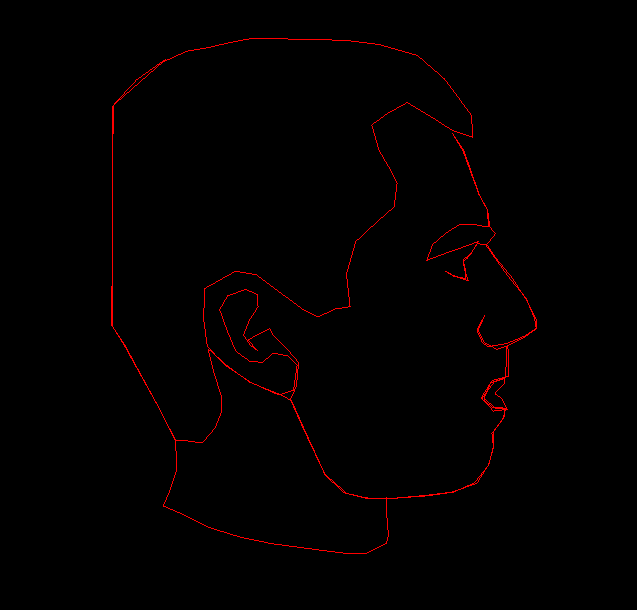
\includegraphics[width=0.45\linewidth]{screenshot.png}
    \caption{Final output}
\end{figure}

\newpage
\lstinputlisting[caption=Python Tracing Program, language=Python, captionpos=t]{../tracer/tracer.py}
\newpage
\lstinputlisting[caption=Full program, captionpos=t]{main.cpp}

\end{document}
